\chapter{Implementations}
In this chapter we dive into the implementation part and discuss different approaches. First, we specify on how the AFs we run the experiments on were created in \cref{sec:ImplementationsCreatingAFs}. Here we describe three different methods, with their advantages and disadvantages. Next we explain two different settings to optimize the spurious/faithful check in \cref{sec:ImplementationsBFSandDFSApproach}. In \cref{sec:ImplementationsGeneratingSemanticsSets} is the explanation on how we generated the semantics extensions and in \cref{sec:ImplementationsFaithfulSpuriousDetermination} we describe the method to determine if an AF is spurious or faithful. Finally, we will tackle refuted theories in \cref{sec:ImplementationsRefutedTheories}.

\section{Creating AFs}
\label{sec:ImplementationsCreatingAFs}
We created three different approaches to generate AFs. Each of them has a different idea and generates AFs with different properties. While the random-based approach generates chaotic AFs, which are typically not similar to real-world problems, the grid-based approach has structure and is therefore more related to real-world problems. The level-based approach has even more structure and assures that we can not derive to many neighbours from a problematic argument. For each approach, we provide an additional figure to visualize it, and also a pseudo-code.

\paragraph{random-based} Let us begin with the random-based approach. The arguments of the script are \texttt{<arg\_amount>} and \texttt{<p>}. The \texttt{<arg\_amount>} specifies how many arguments the AF has and the argument \texttt{<p>} defines the probability of an attack between two arguments. This approach creates chaotic AFs with no structure. Basically, if we take a look at \cref{fig:LevelBasedApproach} we can see a graph with potential attacks depicted with dotted arrows. Every potential attack has a a probability of \texttt{<p>} to be an actual attack of the generated AF.


\begin{figure}[h!]
    \centering
    \begin{tikzpicture}
        \def \rectSize{0.7cm}
        \def \rectSpace{1.8cm}
        
        \node[rectangle, draw, line width=0.3mm, minimum width=\rectSize, minimum height=\rectSize] at (0, 0) {};
        \node[rectangle, draw, line width=0.3mm, minimum width=\rectSize, minimum height=\rectSize] at (\rectSpace, 0) {};
        \node[rectangle, draw, line width=0.3mm, minimum width=\rectSize, minimum height=\rectSize] at (0, \rectSpace) {};
        \node[rectangle, draw, line width=0.3mm, minimum width=\rectSize, minimum height=\rectSize] at (\rectSpace, \rectSpace) {};

        % bottom
        \draw[dotted,<->, line width=0.3mm, >={To[length=4, width=5]}]
        (0 + \rectSize/2, 0) -- (\rectSpace - \rectSize/2, 0);
        % top
        \draw[dotted,<->, line width=0.3mm, >={To[length=4, width=5]}]
        (0 + \rectSize/2, \rectSpace) -- (\rectSpace - \rectSize/2, \rectSpace);
        % left
        \draw[dotted,<->, line width=0.3mm, >={To[length=4, width=5]}]
        (0,0 + \rectSize/2) -- (0, \rectSpace - \rectSize/2);
        % right
        \draw[dotted,<->, line width=0.3mm, >={To[length=4, width=5]}]
        (\rectSpace, 0 + \rectSize/2) -- (\rectSpace , \rectSpace - \rectSize/2);
        % center positive
        \draw[dotted,<->, line width=0.3mm, >={To[length=4, width=5]}]
        (0 + \rectSize/2, 0 + \rectSize/2) -- (\rectSpace - \rectSize/2, \rectSpace-\rectSize/2);
        % center negative
        \draw[dotted,<->, line width=0.3mm, >={To[length=4, width=5]}]
        (0 + \rectSize/2, \rectSpace - \rectSize/2) -- (\rectSpace - \rectSize/2, \rectSize/2);

    \end{tikzpicture}
    \caption{Random-Based Approach. $Amount=4$}
    \label{fig:LevelBasedApproach}
\end{figure}

Random-based generated AFs have the property (depending on the probability value) of being hard to to predict on how good the AF is solvable. This is due the fact, that the neighbours of each argument are highly dependent on the amount of attacks and randomness. Example AFs generated with the random-based approach can be seen in \cref{fig:ImplementationRandomBasedExampleAFs}


\vspace{0.3cm}
\begin{figure}[h]
    \begin{minipage}{.3\textwidth}
        \centering
        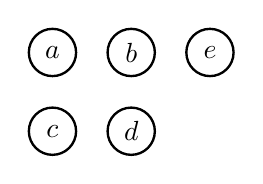
\begin{tikzpicture}
            \def \ax{0}   \def \ay{0}
            \def \bx{1}   \def \by{0}
            \def \cx{0}   \def \cy{-1}
            \def \dx{1}   \def \dy{-1}
            \def \ex{2}   \def \ey{0}

            \draw[line width=0.3mm] (\ax, \ay) circle (0.3) node[anchor=center]{$a$};
            \draw[line width=0.3mm] (\bx, \by) circle (0.3) node[anchor=center]{$b$};
            \draw[line width=0.3mm] (\cx, \cy) circle (0.3) node[anchor=center]{$c$};
            \draw[line width=0.3mm] (\dx, \dy) circle (0.3) node[anchor=center]{$d$};
            \draw[line width=0.3mm] (\ex, \ey) circle (0.3) node[anchor=center]{$e$};
            % Attacks
            \DrawSelfAttackRightSingleton{\ex}{\ey}
            \DrawAttackVertical{B}{\ax}{\ay}{\cx}{\cy}
            \DrawAttackHorizontal{R}{\ax}{\ay}{\bx}{\by}
            \DrawAttackHorizontal{L}{\dx}{\dy}{\cx}{\cy}
            \DrawAttackDiagonal{PLR}{\cx}{\cy}{\bx}{\by}
    
        \end{tikzpicture}
        \subcaption{\texttt{arg\_amount}=5 \texttt{p}=0.25}
        \label{af:ImplementationRandomBasedExampleAFsa}
    \end{minipage}
\begin{minipage}{.3\textwidth}
    \centering
    \begin{tikzpicture}
        % Singletons
        \def \ax{0}   \def \ay{0}
        \def \bx{1}   \def \by{0}
        \def \cx{1}   \def \cy{-1}
        \def \dx{2}   \def \dy{0}
        \def \ex{2}   \def \ey{-1}

        \draw[line width=0.3mm] (\ax, \ay) circle (0.3) node[anchor=center]{$a$};
        \draw[line width=0.3mm] (\bx, \by) circle (0.3) node[anchor=center]{$b$};
        \draw[line width=0.3mm] (\cx, \cy) circle (0.3) node[anchor=center]{$c$};
        \draw[line width=0.3mm] (\dx, \dy) circle (0.3) node[anchor=center]{$d$};
        \draw[line width=0.3mm] (\ex, \ey) circle (0.3) node[anchor=center]{$e$};

        % Attacks
        \DrawSelfAttackLeftSingleton{\ax}{\ay}
        \DrawSelfAttackRightSingleton{\dx}{\dy}
        \DrawSelfAttackRightSingleton{\ex}{\ey}
        \DrawAttackHorizontal{L}{\bx}{\by}{\ax}{\ay}
        \DrawAttackHorizontal{R}{\bx}{\by}{\dx}{\dy}
        \DrawAttackHorizontal{R}{\cx}{\cy}{\ex}{\ey}
        \DrawAttackVertical{D}{\dx}{\dy}{\ex}{\ey}
        \DrawAttackVertical{D}{\bx}{\by}{\cx}{\cy}
        \DrawAttackDiagonal{NLR}{\bx}{\by}{\ex}{\ey}
        \DrawAttackDiagonal{NRL}{\cx}{\cy}{\ax}{\ay}

        % Weird Attack
        \def \argSize{0.3}
        \draw[-{To[length=4, width=5]}, line width=0.3mm]
            (\ax + \argSize/2, \ay + \argSize - 0.05) .. controls
            (\bx-0.2 , \by + \argSize + 0.2) and
            (\bx+0.2 , \by + \argSize + 0.2) ..
            (\dx - \argSize/2, \dy + \argSize - 0.05);
    \end{tikzpicture}
    \subcaption{\texttt{arg\_amount}=5 \texttt{p}=0.5}
    \label{af:ImplementationRandomBasedExampleAFsb}
\end{minipage}%
\begin{minipage}{.3\textwidth}
    \centering
    \begin{tikzpicture}
        % Singletons
        \def \ax{0}   \def \ay{0}
        \def \bx{1}   \def \by{0}
        \def \cx{0}   \def \cy{-1}
        \def \dx{1}   \def \dy{-1}
        \def \ex{2}   \def \ey{0}

        \draw[line width=0.3mm] (\ax, \ay) circle (0.3) node[anchor=center]{$a$};
        \draw[line width=0.3mm] (\bx, \by) circle (0.3) node[anchor=center]{$b$};
        \draw[line width=0.3mm] (\cx, \cy) circle (0.3) node[anchor=center]{$c$};
        \draw[line width=0.3mm] (\dx, \dy) circle (0.3) node[anchor=center]{$d$};
        \draw[line width=0.3mm] (\ex, \ey) circle (0.3) node[anchor=center]{$e$};

        % Attacks
        \DrawSelfAttackLeftSingleton{\ax}{\ay}
        \DrawSelfAttackLeftSingleton{\cx}{\cy}
        \DrawSelfAttackRightSingleton{\ex}{\ey}
        \DrawAttackDiagonal{NB}{\ax}{\ay}{\dx}{\dy}
        \DrawAttackDiagonal{PB}{\bx}{\by}{\cx}{\cy}
        \DrawAttackHorizontal{L}{\bx}{\by}{\ax}{\ay}
        \DrawAttackHorizontal{R}{\cx}{\cy}{\dx}{\dy}
        \DrawAttackHorizontal{L}{\ex}{\ey}{\bx}{\by}
        \DrawAttackVertical{B}{\ax}{\ay}{\cx}{\cy}

        % Weird Attack
        \def \argSize{0.3}
        \draw[-{To[length=4, width=5]}, line width=0.3mm]
            (\ax + \argSize/2, \ay + \argSize - 0.05) .. controls
            (\bx-0.2 , \by + \argSize + 0.2) and
            (\bx+0.2 , \by + \argSize + 0.2) ..
            (\ex - \argSize/2, \ey + \argSize - 0.05);
    \end{tikzpicture}
    \subcaption{\texttt{arg\_amount}=5 \texttt{p}=0.75}
    \label{af:ImplementationRandomBasedExampleAFsc}
\end{minipage}
\caption{Example AF generated with random-based approach}
\label{fig:ImplementationRandomBasedExampleAFs}
\end{figure}
\vspace{0.3cm}



\paragraph{grid-based} Next we are going to discuss the grid-based approach. The arguments for the script are \texttt{<arg\_amount>}, being the amount of arguments the AF has and \texttt{<p>}, which is the probability that an attack between two arguments occurs. Different to the random-based approach, attacks can only happen between the direct neighbours of the grid (i.e.\ top, bottom, right, left). The grid is a $n \times n$ grid, with $n$ being equal to $\lfloor (\sqrt{\texttt{<arg\_amount>}}) \rfloor$. An example grid can be seen in \cref{fig:GridBasedApproach}.

\begin{figure}[h!]
    \centering
    \begin{tikzpicture}
        \def \rectSize{0.7cm}
        \def \rectSpace{0.5cm}

        \foreach \row in {0,1,2,3} {
            \foreach \col in {0,1,2,3} {
                \def \x{\rectSize * \col + \rectSpace * \col}
                \def \y{\rectSize * \row + \rectSpace * \row}
                \def \xArrowStart{\x+\rectSize/2}
                \def \xArrowEnd{\x+\rectSize/2+\rectSpace}
                \def \yArrowStart{\y+\rectSize/2}
                \def \yArrowEnd{\y+\rectSize/2+\rectSpace}

                % Rectangle
                \node[rectangle, draw, line width=0.3mm, minimum width=\rectSize, minimum height=\rectSize] at (\x, \y) {};

                \ifnum\col<3
                    % Arrow
                    \draw[dotted,<->, line width=0.3mm, >={To[length=4, width=5]}] (\xArrowStart,\y) -- (\xArrowEnd,\y);
                \fi

                \ifnum\row<3
                    % Arrow
                    \draw[dotted,<->, line width=0.3mm, >={To[length=4, width=5]}] (\x,\yArrowStart) -- (\x,\yArrowEnd);
                \fi
            }
        }
    \end{tikzpicture}
    \caption{Grid-Based Approach. $Amount=16$}
    \label{fig:GridBasedApproach}
\end{figure}

With the grid-based approach, we obtain a more structured AF. Structured in this context means, that the attacks between the arguments are restricted to locality. Due to this restriction, we reduce the amount of neighbours drastically in comparison to the random-based approach. Since we have less neighbours, we decrease the computation time and increase the chance to find a faithful AF. Example AF created with the grid-based approach can be seen in \cref{fig:ImplementationGridBasedExampleAFs}.



\vspace{0.3cm}
\begin{figure}[h]
    \begin{minipage}{.3\textwidth}
        \centering
        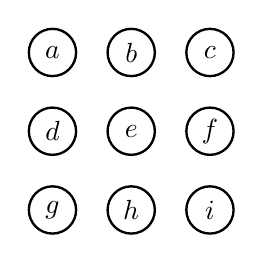
\begin{tikzpicture}
            \def \ax{0}   \def \ay{0}
            \def \bx{1}   \def \by{0}
            \def \cx{2}   \def \cy{0}
            \def \dx{0}   \def \dy{-1}
            \def \ex{1}   \def \ey{-1}
            \def \fx{2}   \def \fy{-1}
            \def \gx{0}   \def \gy{-2}
            \def \hx{1}   \def \hy{-2}
            \def \ix{2}   \def \iy{-2}

            \draw[line width=0.3mm] (\ax, \ay) circle (0.3) node[anchor=center]{$a$};
            \draw[line width=0.3mm] (\bx, \by) circle (0.3) node[anchor=center]{$b$};
            \draw[line width=0.3mm] (\cx, \cy) circle (0.3) node[anchor=center]{$c$};
            \draw[line width=0.3mm] (\dx, \dy) circle (0.3) node[anchor=center]{$d$};
            \draw[line width=0.3mm] (\ex, \ey) circle (0.3) node[anchor=center]{$e$};
            \draw[line width=0.3mm] (\fx, \fy) circle (0.3) node[anchor=center]{$f$};
            \draw[line width=0.3mm] (\gx, \gy) circle (0.3) node[anchor=center]{$g$};
            \draw[line width=0.3mm] (\hx, \hy) circle (0.3) node[anchor=center]{$h$};
            \draw[line width=0.3mm] (\ix, \iy) circle (0.3) node[anchor=center]{$i$};
            % Attacks
            \DrawAttackHorizontal{R}{\ax}{\ay}{\bx}{\by}
            \DrawAttackHorizontal{R}{\dx}{\dy}{\ex}{\ey}
            \DrawAttackHorizontal{R}{\bx}{\by}{\cx}{\cy}
            \DrawAttackVertical{U}{\ex}{\ey}{\bx}{\by}
            \DrawAttackVertical{B}{\ex}{\ey}{\hx}{\hy}
            \DrawAttackHorizontal{L}{\ix}{\iy}{\hx}{\hy}


        \end{tikzpicture}
        \subcaption{\texttt{arg\_amount}=9 \texttt{p}=0.25}
        \label{af:ImplementationGridBasedExampleAFsa}
    \end{minipage}
\begin{minipage}{.3\textwidth}
    \centering
    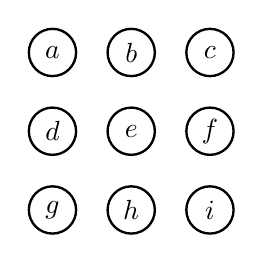
\begin{tikzpicture}
        \def \ax{0}   \def \ay{0}
        \def \bx{1}   \def \by{0}
        \def \cx{2}   \def \cy{0}
        \def \dx{0}   \def \dy{-1}
        \def \ex{1}   \def \ey{-1}
        \def \fx{2}   \def \fy{-1}
        \def \gx{0}   \def \gy{-2}
        \def \hx{1}   \def \hy{-2}
        \def \ix{2}   \def \iy{-2}

        \draw[line width=0.3mm] (\ax, \ay) circle (0.3) node[anchor=center]{$a$};
        \draw[line width=0.3mm] (\bx, \by) circle (0.3) node[anchor=center]{$b$};
        \draw[line width=0.3mm] (\cx, \cy) circle (0.3) node[anchor=center]{$c$};
        \draw[line width=0.3mm] (\dx, \dy) circle (0.3) node[anchor=center]{$d$};
        \draw[line width=0.3mm] (\ex, \ey) circle (0.3) node[anchor=center]{$e$};
        \draw[line width=0.3mm] (\fx, \fy) circle (0.3) node[anchor=center]{$f$};
        \draw[line width=0.3mm] (\gx, \gy) circle (0.3) node[anchor=center]{$g$};
        \draw[line width=0.3mm] (\hx, \hy) circle (0.3) node[anchor=center]{$h$};
        \draw[line width=0.3mm] (\ix, \iy) circle (0.3) node[anchor=center]{$i$};
        % Attacks
        \DrawAttackHorizontal{R}{\ax}{\ay}{\bx}{\by}
        \DrawAttackHorizontal{R}{\dx}{\dy}{\ex}{\ey}
        \DrawAttackHorizontal{R}{\bx}{\by}{\cx}{\cy}
        \DrawAttackHorizontal{L}{\fx}{\fy}{\ex}{\ey}
        \DrawAttackHorizontal{B}{\hx}{\hy}{\gx}{\gy}
        \DrawAttackVertical{U}{\gx}{\gy}{\dx}{\dy}
        \DrawAttackVertical{D}{\cx}{\cy}{\fx}{\fy}
        \DrawAttackVertical{U}{\ex}{\ey}{\bx}{\by}
        \DrawAttackVertical{B}{\ax}{\ay}{\dx}{\dy}
        \DrawAttackVertical{B}{\fx}{\fy}{\ix}{\iy}

    \end{tikzpicture}
    \subcaption{\texttt{arg\_amount}=9 \texttt{p}=0.5}
    \label{af:ImplementationGridBasedExampleAFsb}
\end{minipage}%
\begin{minipage}{.3\textwidth}
    \centering
    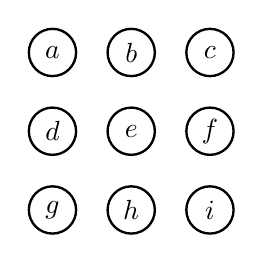
\begin{tikzpicture}
        \def \ax{0}   \def \ay{0}
        \def \bx{1}   \def \by{0}
        \def \cx{2}   \def \cy{0}
        \def \dx{0}   \def \dy{-1}
        \def \ex{1}   \def \ey{-1}
        \def \fx{2}   \def \fy{-1}
        \def \gx{0}   \def \gy{-2}
        \def \hx{1}   \def \hy{-2}
        \def \ix{2}   \def \iy{-2}

        \draw[line width=0.3mm] (\ax, \ay) circle (0.3) node[anchor=center]{$a$};
        \draw[line width=0.3mm] (\bx, \by) circle (0.3) node[anchor=center]{$b$};
        \draw[line width=0.3mm] (\cx, \cy) circle (0.3) node[anchor=center]{$c$};
        \draw[line width=0.3mm] (\dx, \dy) circle (0.3) node[anchor=center]{$d$};
        \draw[line width=0.3mm] (\ex, \ey) circle (0.3) node[anchor=center]{$e$};
        \draw[line width=0.3mm] (\fx, \fy) circle (0.3) node[anchor=center]{$f$};
        \draw[line width=0.3mm] (\gx, \gy) circle (0.3) node[anchor=center]{$g$};
        \draw[line width=0.3mm] (\hx, \hy) circle (0.3) node[anchor=center]{$h$};
        \draw[line width=0.3mm] (\ix, \iy) circle (0.3) node[anchor=center]{$i$};
        % Attacks
        \DrawAttackHorizontal{B}{\bx}{\by}{\ax}{\ay}
        \DrawAttackHorizontal{B}{\ex}{\ey}{\dx}{\dy}
        \DrawAttackHorizontal{B}{\cx}{\cy}{\bx}{\by}
        \DrawAttackHorizontal{B}{\ix}{\iy}{\hx}{\hy}
        \DrawAttackHorizontal{R}{\ex}{\ey}{\fx}{\fy}
        \DrawAttackHorizontal{L}{\hx}{\hy}{\gx}{\gy}
        \DrawAttackVertical{B}{\bx}{\by}{\ex}{\ey}
        \DrawAttackVertical{B}{\fx}{\fy}{\ix}{\iy}
        \DrawAttackVertical{B}{\dx}{\dy}{\gx}{\gy}
        \DrawAttackVertical{D}{\ex}{\ey}{\hx}{\hy}
        \DrawAttackVertical{B}{\ax}{\ay}{\dx}{\dy}
        \DrawAttackVertical{U}{\fx}{\fy}{\cx}{\cy}
    \end{tikzpicture}
    \subcaption{\texttt{arg\_amount}=9 \texttt{p}=0.75}
    \label{af:ImplementationGridBasedExampleAFsc}
\end{minipage}
\caption{Example AF generated with grid-based approach}
\label{fig:ImplementationGridBasedExampleAFs}
\end{figure}
\vspace{0.3cm}



\paragraph{level-based} The last approach we provide is the level-based approach. The arguments for this script are \texttt{<arg\_amount>}, \texttt{<level>} and \texttt{<p>}. Same as for the grid-based and random-based approach, \texttt{<arg\_amount>} defines how many arguments the computed AF has. The \texttt{<level>} argument restricts the height of the grid to the provided value and \texttt{<p>} is again the probability that an attack between to arguments occurs. The difference to the grid-based approach is the dimension of the grid. While the grid-based approach uses a $n \times n$ grid, in the level-based approach we use a $\texttt{<level>} \times n$ grid. In this context, $n$ is equal to $\lceil \texttt{<arg\_amount>}/2 \rceil$. An example grid is depicted in \cref{fig:LevelBasedApproach}.


\begin{figure}[h!]
    \centering
    \begin{tikzpicture}
        \def \rectSize{0.7cm}
        \def \rectSpace{0.5cm}

        \foreach \row in {0,1} {
            \foreach \col in {0,1,2,3,4,5,6,7} {
                \def \x{\rectSize * \col + \rectSpace * \col}
                \def \y{\rectSize * \row + \rectSpace * \row}
                \def \xArrowStart{\x+\rectSize/2}
                \def \xArrowEnd{\x+\rectSize/2+\rectSpace}
                \def \yArrowStart{\y+\rectSize/2}
                \def \yArrowEnd{\y+\rectSize/2+\rectSpace}

                % Rectangle
                \node[rectangle, draw, line width=0.3mm, minimum width=\rectSize, minimum height=\rectSize] at (\x, \y) {};

                \ifnum\col<7
                    % Arrow
                    \draw[dotted,<->, line width=0.3mm, >={To[length=4, width=5]}] (\xArrowStart,\y) -- (\xArrowEnd,\y);
                \fi

                \ifnum\row<1
                    % Arrow
                    \draw[dotted,<->, line width=0.3mm, >={To[length=4, width=5]}] (\x,\yArrowStart) -- (\x,\yArrowEnd);
                \fi
            }
        }
    \end{tikzpicture}
    \caption{Level-Based Approach. $Level=2$ and $Amount=16$}
    \label{fig:LevelBasedApproach}
\end{figure}


With the level-based approach, we obtain the same structured AF as for the grid-based, but with less neighbours. Every argument can only have $min(\texttt{<level>}+1, 4)$ amount of direct neighbours. This reduces the neighbours even further and thus, decreases the overall computation effort. Example AFs created with the level-based script can be seen in \cref{fig:ImplementationLevelBasedExampleAFs}


\vspace{0.3cm}
\begin{figure}[h]
    \begin{minipage}{.5\textwidth}
        \centering
        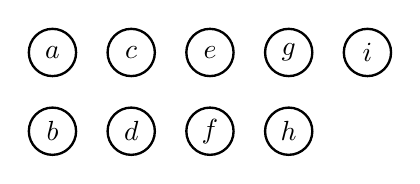
\begin{tikzpicture}
            \def \ax{0}   \def \ay{0}
            \def \bx{0}   \def \by{-1}
            \def \cx{1}   \def \cy{0}
            \def \dx{1}   \def \dy{-1}
            \def \ex{2}   \def \ey{0}
            \def \fx{2}   \def \fy{-1}
            \def \gx{3}   \def \gy{0}
            \def \hx{3}   \def \hy{-1}
            \def \ix{4}   \def \iy{0}

            \draw[line width=0.3mm] (\ax, \ay) circle (0.3) node[anchor=center]{$a$};
            \draw[line width=0.3mm] (\bx, \by) circle (0.3) node[anchor=center]{$b$};
            \draw[line width=0.3mm] (\cx, \cy) circle (0.3) node[anchor=center]{$c$};
            \draw[line width=0.3mm] (\dx, \dy) circle (0.3) node[anchor=center]{$d$};
            \draw[line width=0.3mm] (\ex, \ey) circle (0.3) node[anchor=center]{$e$};
            \draw[line width=0.3mm] (\fx, \fy) circle (0.3) node[anchor=center]{$f$};
            \draw[line width=0.3mm] (\gx, \gy) circle (0.3) node[anchor=center]{$g$};
            \draw[line width=0.3mm] (\hx, \hy) circle (0.3) node[anchor=center]{$h$};
            \draw[line width=0.3mm] (\ix, \iy) circle (0.3) node[anchor=center]{$i$};
            % Attacks
            \DrawAttackHorizontal{R}{\ax}{\ay}{\cx}{\cy}
            \DrawAttackHorizontal{R}{\fx}{\fy}{\hx}{\hy}
            \DrawAttackHorizontal{R}{\dx}{\dy}{\fx}{\fy}
            \DrawAttackHorizontal{L}{\gx}{\gy}{\ex}{\ey}
            \DrawAttackVertical{D}{\ax}{\ay}{\bx}{\by}
            \DrawAttackVertical{B}{\gx}{\gy}{\hx}{\hy}
        \end{tikzpicture}
        \subcaption{\texttt{arg\_amount}=9 \texttt{level}=2 \texttt{p}=0.25}
        \label{af:ImplementationLevelBasedExampleAFsa}
    \end{minipage}
\begin{minipage}{.5\textwidth}
    \centering
    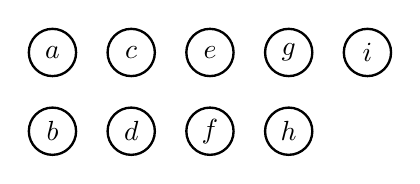
\begin{tikzpicture}
        \def \ax{0}   \def \ay{0}
        \def \bx{0}   \def \by{-1}
        \def \cx{1}   \def \cy{0}
        \def \dx{1}   \def \dy{-1}
        \def \ex{2}   \def \ey{0}
        \def \fx{2}   \def \fy{-1}
        \def \gx{3}   \def \gy{0}
        \def \hx{3}   \def \hy{-1}
        \def \ix{4}   \def \iy{0}

        \draw[line width=0.3mm] (\ax, \ay) circle (0.3) node[anchor=center]{$a$};
        \draw[line width=0.3mm] (\bx, \by) circle (0.3) node[anchor=center]{$b$};
        \draw[line width=0.3mm] (\cx, \cy) circle (0.3) node[anchor=center]{$c$};
        \draw[line width=0.3mm] (\dx, \dy) circle (0.3) node[anchor=center]{$d$};
        \draw[line width=0.3mm] (\ex, \ey) circle (0.3) node[anchor=center]{$e$};
        \draw[line width=0.3mm] (\fx, \fy) circle (0.3) node[anchor=center]{$f$};
        \draw[line width=0.3mm] (\gx, \gy) circle (0.3) node[anchor=center]{$g$};
        \draw[line width=0.3mm] (\hx, \hy) circle (0.3) node[anchor=center]{$h$};
        \draw[line width=0.3mm] (\ix, \iy) circle (0.3) node[anchor=center]{$i$};
        % Attacks
        \DrawAttackHorizontal{B}{\cx}{\cy}{\ax}{\ay}
        \DrawAttackHorizontal{B}{\hx}{\hy}{\fx}{\fy}
        \DrawAttackHorizontal{B}{\ex}{\ey}{\cx}{\cy}
        \DrawAttackHorizontal{B}{\ix}{\iy}{\gx}{\gy}
        \DrawAttackHorizontal{R}{\dx}{\dy}{\fx}{\fy}
        \DrawAttackHorizontal{R}{\ex}{\ey}{\gx}{\gy}
        \DrawAttackHorizontal{L}{\dx}{\dy}{\bx}{\by}
        \DrawAttackVertical{U}{\bx}{\by}{\ax}{\ay}
        \DrawAttackVertical{D}{\gx}{\gy}{\hx}{\hy}
        \DrawAttackVertical{B}{\cx}{\cy}{\dx}{\dy}
        \DrawAttackVertical{B}{\ex}{\ey}{\fx}{\fy}
    \end{tikzpicture}
    \subcaption{\texttt{arg\_amount}=9 \texttt{level}=2 \texttt{p}=0.75}
    \label{af:ImplementationLevelBasedExampleAFsb}
\end{minipage}%
\caption{Example AF generated with grid-based approach}
\label{fig:ImplementationLevelBasedExampleAFs}
\end{figure}
\vspace{0.3cm}

\paragraph{clustering} Todo


\newpage
\section{BFS and DFS Approach}
\label{sec:ImplementationsBFSandDFSApproach}
Breadth-First-Search (BFS) and Depth-First-Search (DFS) are usually used in algorithms to traverse graphs. Where BFS visits each node in order of distance to the start, DFS follows a direct path and only backtracks, if is has to. We, however, are not using the two approaches to traverse a graph, but we are using a similar principle to compute faithfulness of an abstract AF. The BFS approach in our implementation first computes all the semantics extensions of the abstract AF, then computes all the semantics extensions of the concrete AF and finally compares them to check for spuriousness.

\begin{figure}[h!]
    \centering
    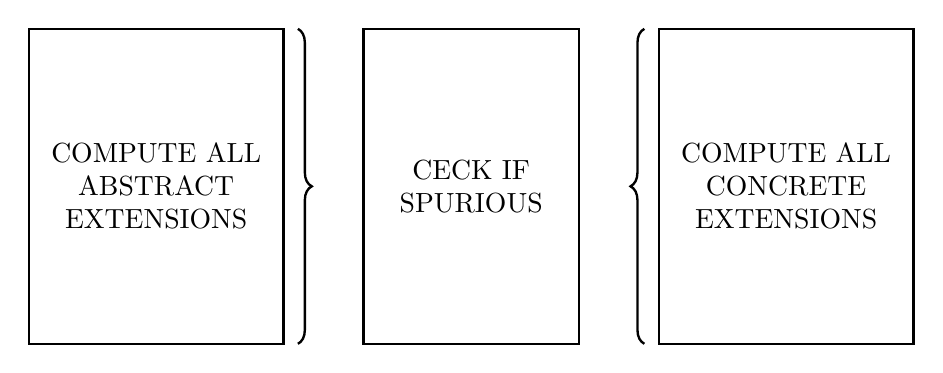
\begin{tikzpicture}
        % Compute Block
        \def \computeBlockX{0}
        \def \computeBlockY{0}
        \def \computeBlockWidth{3cm}
        \def \computeBlockHeight{4cm}
        \node[rectangle, draw, line width=0.3mm, minimum width=\computeBlockWidth, minimum height=\computeBlockHeight , text width=\computeBlockWidth, align=center] at (\computeBlockX, \computeBlockY) {COMPUTE ALL ABSTRACT EXTENSIONS};


        % Check Block
        \def \checkBlockX{4}
        \def \checkBlockY{0}
        \def \checkBlockWidth{2.5cm}
        \def \checkBlockHeight{4cm}
        \node[rectangle, draw, line width=0.3mm, minimum width=\checkBlockWidth, minimum height=\checkBlockHeight , text width=\checkBlockWidth, align=center] at (\checkBlockX, \checkBlockY) {CECK IF SPURIOUS};
        
        % Brace
        \draw [line width=0.3mm, decorate, decoration = {brace, amplitude=5pt, mirror}] (1.8,-2) --  (1.8,2);
        \DrawAttackHorizontal{R}{1.7}{0}{2.9}{0}

        \draw [line width=0.3mm, decorate, decoration = {brace, amplitude=5pt}] (6.2,-2) --  (6.2,2);
        \DrawAttackHorizontal{L}{6.3}{0}{5.1}{0}

        % Compute Block
        \def \compBlockX{8}
        \def \compBlockY{0}
        \def \compBlockWidth{3cm}
        \def \compBlockHeight{4cm}
        \node[rectangle, draw, line width=0.3mm, minimum width=\compBlockWidth, minimum height=\compBlockHeight , text width=\compBlockWidth, align=center] at (\compBlockX, \compBlockY) {COMPUTE ALL CONCRETE EXTENSIONS};
    \end{tikzpicture}
    \caption{BFS visualization}
    \label{fig:ImplementationBFSVisualization}
\end{figure}



The BFS approach, visualized in \cref{fig:ImplementationBFSVisualization} is practical for AFs which do not have many semantics extensions. If the semantics sets take too long to compute, we will run into a timeout no matter at which seed the SAT-Solver is operating on. BFS is a solid and robust approach, nevertheless, there is no space of randomness and lucky early terminations.

On the other hand, we have the DFS approach depicted in \cref{fig:ImplementationDFSVisualization}. When using DFS, instead of calculating all the abstract extensions at once, we verify each computed set directly. Verifying in this context means, to check if the extension can be mapped to one of the concrete extensions. But instead of computing every possible concrete set, and checking for a valid mapping, we encode the extensions directly, add a new context (using incremental solving), and check for satisfiability. If the SAT-Solver returns \emph{UNSAT}, we found a spurious extension and, therefore, showed that the abstract AF is spurious.


\begin{figure}[h]
    \centering
    \begin{tikzpicture}
        \def \bwidth{3cm}
        \def \bheight{1.5cm}
        % Block 1
        \def \cbIX{0}
        \def \cbIY{1.5cm}
        \node[rectangle, draw, line width=0.3mm, minimum width=\bwidth, minimum height=\bheight , text width=\bwidth, align=center] at (\cbIX, \cbIY) {COMPUTE ABSTRACT EXTENSION};

        % Block connection dotted
        \draw[dotted,-, line width=0.5mm, >={To[length=4, width=5]}]
        (0cm, 0.45cm) -- (0cm, -0.45cm);

        % Block 2
        \def \cbIIX{0}
        \def \cbIIY{-1.5cm}
        \node[rectangle, draw, line width=0.3mm, minimum width=\bwidth, minimum height=\bheight , text width=\bwidth, align=center] at (\cbIIX, \cbIIY) {COMPUTE ABSTRACT EXTENSION};



        % Block 3
        \def \cbIIIX{4}
        \def \cbIIIY{1.5cm}
        \node[rectangle, draw, line width=0.3mm, minimum width=\bwidth, minimum height=\bheight , text width=\bwidth, align=center] at (\cbIIIX, \cbIIIY) {VERIFY ON CONCRETE AF};
        \DrawAttackHorizontal{R}{1.3}{1.5cm}{2.7}{1.5cm}

        % Block connection dotted
        \draw[dotted,-, line width=0.5mm, >={To[length=4, width=5]}]
        (4.2cm, 0.45cm) -- (4.2cm, -0.45cm);

        % Block 4
        \def \cbIIIIX{4}
        \def \cbIIIIY{-1.5cm}
        \node[rectangle, draw, line width=0.3mm, minimum width=\bwidth, minimum height=\bheight , text width=\bwidth, align=center] at (\cbIIIIX, \cbIIIIY) {VERIFY ON CONCRETE AF};
        \DrawAttackHorizontal{R}{1.3}{-1.5cm}{2.7}{-1.5cm}


        % Brace
        \draw [line width=0.3mm, decorate, decoration = {brace, amplitude=5pt, mirror}] (5.8,-2.25) --  (5.8,2.25);
        \DrawAttackHorizontal{R}{5.7}{0}{6.9}{0}

        % Check Block
        \def \checkBlockX{8}
        \def \checkBlockY{0}
        \def \checkBlockWidth{2.5cm}
        \def \checkBlockHeight{4cm}
        \node[rectangle, draw, line width=0.3mm, minimum width=\checkBlockWidth, minimum height=\checkBlockHeight , text width=\checkBlockWidth, align=center] at (\checkBlockX, \checkBlockY) {IF ANY VERIFY BLOCK IS UNSAT, RETURN SPURIOUS};
    \end{tikzpicture}
    \caption{DFS visualization}
    \label{fig:ImplementationDFSVisualization}
\end{figure}


DFS has some overhead, due to the context switches resulting with a longer computation power for faithful AFs. Nevertheless, depending on the seed of the SAT-Solver, we can obtain a result much faster than with BFS. If the first computed semantics extension is already spurious, we save a lot of computation power and can even solve AFs, which are not feasible for the BFS approach.







\section{Generating Semantics Sets}
\label{sec:ImplementationsGeneratingSemanticsSets}

To be able to create semantics extensions with a SAT-Solver, we need to encode the semantics (previously defined in \cref{sec:Encodings} and the according refinements in \cref{sec:HeuristicsAndRefinements}) into Boolean logic. Since the semantics definitions are written in an generelazide form, we need to unpack the n-ary con-/disjunction and encode them appropriately.


\begin{example}
Let us have a look at a concrete example with an abstract clustered AF $\hat{G}=(\hat{A}, \hat{R})$ defined in \cref{af:implementationSATExample1}. The arguments of the AF are $\hat{A}=\{c, d, e, \hat{h}\}$, with the cluster $\hat{h}$ containing the arguments $\{a, b\}$ and the rules being $\hat{R}=\bigl\{ (\hat{h}, c)$, $(c, c)$, $(c, d)$, $(c, e)$, $(e, d)$, $(d, e)\bigl\}$.

\begin{figure}[h]
    \centering
    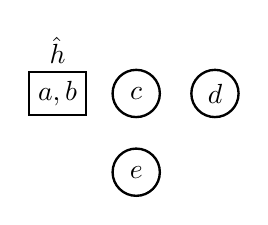
\begin{tikzpicture}
        % Singletons
        \def \cx{1}     \def \cy{0}
        \def \dx{2}     \def \dy{0}
        \def \ex{1}     \def \ey{-1}
        \def \hx{0}     \def \hy{0}

        \node[rectangle, draw, line width=0.3mm] at (\hx, \hy) {$a,b$};
        \node at (0, 0.55) {$\hat{h}$};
        \draw[line width=0.3mm] (\cx, \cy) circle (0.3) node[anchor=center]{$c$};
        \draw[line width=0.3mm] (\dx, \dy) circle (0.3) node[anchor=center]{$d$};
        \draw[line width=0.3mm] (\ex, \ey) circle (0.3) node[anchor=center]{$e$};

        % Attacks
        \DrawAttackHorizontal{R}{\hx+0.1}{\hy}{\cx}{\cy}
        \DrawSelfAttackRightSingleton{\cx}{\cy}
        \DrawAttackHorizontal{R}{\cx}{\cy}{\dx}{\dy}
        \DrawAttackVertical{D}{\cx}{\cy}{\ex}{\ey}
        \DrawAttackDiagonal{PB}{\dx}{\dy}{\ex}{\ey}
    \end{tikzpicture}
    \caption{Abstract AF $\hat{G}$}
    \label{af:implementationSATExample1}
\end{figure}


\paragraph{n-ary conjunction} To concatinate all the arguments with a Boolean AND of the AF \emph{$\hat{G}$}, we use the n-ary conjunction operator. We select an argument \emph{a} from the singletons of the AF \emph{$\hat{G}$} and concatinate them conjunctively. Note, that with the subscript \emph{SINGLE} we only include the singletons of the AF.

$$
\bigwedge_{a \in \hat{G}_{\!S\!I\!N\!G\!L\!E}} a = c \land d \land e
$$


\paragraph{n-ary disjunction} To concatinate all the arguments of the AF \emph{$\hat{G}$} with a Boolean OR, we use the n-ary disjunction operator. By iterating over all the arguments of the AF \emph{$\hat{G}$} and concatinating them disjunctively we generate the Boolean formula for the SAT-Solver. Note, that this time we do not have the subscript \emph{SINGLE}, so we include the clusters as well.

$$
\bigvee_{a \in \hat{G}} a = c \lor d \lor e \lor \hat{h}
$$

\paragraph{iterating attacks} We can also iterate over every attack of the AF $\hat{G}$. We can extract both arguments \emph{a} (being the attacker) and \emph{b} (being the defender) from the attacks by selecting the tuples from \emph{$\hat{R}$}.

$$
\bigwedge_{(a, b) \in \hat{R}, a\in \hat{G}_{\!S\!I\!N\!G\!L\!E}} \big( a \lor b \big) = (c \lor c) \land
(c \lor d) \land (c \lor e) \land (e \lor d) \land (d \lor e)
$$
\end{example}

With this encoding, we can compute a model with the SAT-Solver and extract a semantics set. If we try to compute another extension, we first have to add a new Boolean rule. This rule removes the previously found model from the satisfiable solutions by adding the negated disjunction of the arguments from the extension. Or formally, if $S$ is the previously found extension, we add the following formula conjunctively to the previous rule set.

$$
\bigvee_{a \in S} \lnot a
$$


\section{Faithful/Spurious Determination}
\label{sec:ImplementationsFaithfulSpuriousDetermination}
\textit{TODO: Determine faithful/spurious algorithm}

\section{Refuted Theories}
\label{sec:ImplementationsRefutedTheories}
\textit{TODO: State refuted theories like subsets of spurious also spurious.}




